%%%%%%%%%%%%%%%%%%%%%%%%%%%%%%%%%%%%%%%%%%%%%%%%%%%%%%%%%%%%%%%%%%%%%%%%%%%%%%%
%                       CARGA DE LA CLASE DE DOCUMENTO                        %
%                                                                             %
% Las opciones admisibles son:                                                %
%      12pt / 11pt            (tamaño del cuerpo de letra; no usar 10pt)      %
%                                                                             %
% catalan/spanish/english     (idioma principal del trabajo)                  %
%                                                                             % 
% french/italian/german...    (si necesitáis usar otro idioma adicional)      %
%                                                                             %
% listoffigures               (El documento incluye un Índice de figuras)     %
% listoftables                (El documento incluye un Índice de tablas)      %
% listofquadres               (El documento incluye un Índice de cuadros)     %
% listofalgorithms            (El documento incluye un Índice de algoritmos)  %
%                                                                             %
%%%%%%%%%%%%%%%%%%%%%%%%%%%%%%%%%%%%%%%%%%%%%%%%%%%%%%%%%%%%%%%%%%%%%%%%%%%%%%%

\documentclass[11pt,spanish,listoffigures,listoftables]{tfgetsinf}

%%%%%%%%%%%%%%%%%%%%%%%%%%%%%%%%%%%%%%%%%%%%%%%%%%%%%%%%%%%%%%%%%%%%%%%%%%%%%%%
%                     CODIFICACIÓN DEL ARCHIVO FUENTE                         %
%                                                                             %
%    Windows suele usar 'ansinew'                                             %
%    en Linux es posible que sea 'latin1' o 'latin9'                          %
%    Pero lo más recomendable es usar utf8 (unicode 8)                        %
%                                          (si vuestro editor lo permite)     % 
%%%%%%%%%%%%%%%%%%%%%%%%%%%%%%%%%%%%%%%%%%%%%%%%%%%%%%%%%%%%%%%%%%%%%%%%%%%%%%%

\usepackage[utf8]{inputenc} 


%%%%%%%%%%%%%%%%%%%%%%%%%%%%%%%%%%%%%%%%%%%%%%%%%%%%%%%%%%%%%%%%%%%%%%%%%%%%%%%
%                       OTROS PAQUETES Y DEFINICIONES                         %
%                                                                             %
%%%%%%%%%%%%%%%%%%%%%%%%%%%%%%%%%%%%%%%%%%%%%%%%%%%%%%%%%%%%%%%%%%%%%%%%%%%%%%%

\usepackage{glossaries}
\usepackage{textcomp}
\usepackage{booktabs}
\usepackage{float}
\usepackage{enumitem}
\usepackage{graphicx}
\usepackage{subcaption}
\usepackage{tabularx}
\usepackage{pgfplots}
\pgfplotsset{compat=1.18}

% Listings para código
\usepackage{listings}
\lstset{
  basicstyle=\ttfamily\small,
  frame=single,
  breaklines=true,
  postbreak=\mbox{\textcolor{gray}{$\hookrightarrow$}\space},
  columns=fullflexible,
  keepspaces=true,
  numbers=none,
  literate={á}{{\'a}}1 {é}{{\'e}}1 {í}{{\'i}}1 {ó}{{\'o}}1 {ú}{{\'u}}1
           {Á}{{\'A}}1 {É}{{\'E}}1 {Í}{{\'I}}1 {Ó}{{\'O}}1 {Ú}{{\'U}}1
           {ñ}{{\~n}}1 {Ñ}{{\~N}}1 {¿}{{?`}}1 {¡}{{!`}}1
           {ã}{{\~a}}1 {õ}{{\~o}}1 {ê}{{\^e}}1 {ô}{{\^o}}1 {ç}{{\c{c}}}1
}

% Bibliografía
\usepackage[backend=biber,style=numeric,sorting=none]{biblatex}
\addbibresource{bibliografia.bib}

% Hyperref siempre al final
\usepackage{hyperref}
\hypersetup{
  colorlinks=true,
  linkcolor=black,
  urlcolor=cyan,
  citecolor=black
}
%%%%%%%%%%%%%%%%%%%%%%%%%%%%%%%%%%%%%%%%%%%%%%%%%%%%%%%%%%%%%%%%%%%%%%%%%%%%%%%
%                          DATOS DEL TRABAJO                                  %
%                                                                             %
% título alumno, tutor y curso académico                                      %
%%%%%%%%%%%%%%%%%%%%%%%%%%%%%%%%%%%%%%%%%%%%%%%%%%%%%%%%%%%%%%%%%%%%%%%%%%%%%%%

\title{Transcripción-Traducción automática portugués-inglés con Whisper}
\author{Gómez Corral, Miquel}
% \tutor{}
% \curs{MUIARFID}

%%%%%%%%%%%%%%%%%%%%%%%%%%%%%%%%%%%%%%%%%%%%%%%%%%%%%%%%%%%%%%%%%%%%%%%%%%%%%%%
%                     PARAULES CLAU/PALABRAS CLAVE/KEY WORDS                  %
%                                                                             %
% Independentment de la llengua del treball, s'hi han d'incloure              %
% les paraules clau i el resum en els tres idiomes                            %
%%%%%%%%%%%%%%%%%%%%%%%%%%%%%%%%%%%%%%%%%%%%%%%%%%%%%%%%%%%%%%%%%%%%%%%%%%%%%%%

\keywords{
    Traducció de textos; Portuguès; Anglès; Transformers; Whisper;
} % Paraules clau 
{
   Traducción de textos; Portugués; Inglés; Transformers; Whisper;
} % Palabras clave
{
    Speech Translation; Portuguese; English; Transformers; Whisper.
} % Key words


%%%%%%%%%%%%%%%%%%%%%%%%%%%%%%%%%%%%%%%%%%%%%%%%%%%%%%%%%%%%%%%%%%%%%%%%%%%%%%%
%                                                                             %
%                              INICI DEL DOCUMENT                             %
%                                                                             %
%%%%%%%%%%%%%%%%%%%%%%%%%%%%%%%%%%%%%%%%%%%%%%%%%%%%%%%%%%%%%%%%%%%%%%%%%%%%%%%

\begin{document} 


%%%%%%%%%%%%%%%%%%%%%%%%%%%%%%%%%%%%%%%%%%%%%%%%%%%%%%%%%%%%%%%%%%%%%%%%%%%%%%%
%              RESUMENES DEL TFG EN VALENCIA, CASTELLA I ANGLES               %
%%%%%%%%%%%%%%%%%%%%%%%%%%%%%%%%%%%%%%%%%%%%%%%%%%%%%%%%%%%%%%%%%%%%%%%%%%%%%%%


% \begin{abstract}[spanish]

% \end{abstract}

%%%%%%%%%%%%%%%%%%%%%%%%%%%%%%%%%%%%%%%%%%%%%%%%%%%%%%%%%%%%%%%%%%%%%%%%%%%%%%%
%                                                                             %
%                              CONTENIDO DEL TRABAJO                          %
%                                                                             %
%%%%%%%%%%%%%%%%%%%%%%%%%%%%%%%%%%%%%%%%%%%%%%%%%%%%%%%%%%%%%%%%%%%%%%%%%%%%%%%

%%%%%%%%%%%%%%%%%%%%%%%%%%%%%%%%%%%%%%%%%%%%%%%%%%%%%%%%%%%%%%%%%%%%%%%%%%%%%%%
%                                  ÍNDICE                                     %
%%%%%%%%%%%%%%%%%%%%%%%%%%%%%%%%%%%%%%%%%%%%%%%%%%%%%%%%%%%%%%%%%%%%%%%%%%%%%%%
% \clearpage
% \tableofcontents
% \listoffigures
% \listoftables


\mainmatter

\chapter{Introducción}
Este trabajo aborda el uso de modelos 'Whisper' \cite{radford2023robust} para la transcripción y traducción automática de audios en portugués a texto en inglés. 

Se han realizado experimentos a partir del material provisto por la asignatura en formato notebook. Estos experimentos se han llevado a cabo con el dataset \textbf{Covost2-PT-EN}, que contiene frases en portugués y sus correspondientes traducciones al inglés. Son 9158 datos de \textit{train}, 3318 datos de \textit{dev} y 4023 datos de \textit{test} lo que en total hacen 16499 ejemplos.

Se han realizado experimentos de traducción directamente usando Whisper, así como experimentos en cascada usando las transcripciones de Whisper como entrada para un modelo de traducción automática basado en Transformers.


\subsubsection{Hardware utilizado}
Los experimentos se han realizado en mi máquina personal con las siguientes características: GPU NVIDIA RTX 5070 (12 GB VRAM), procesador AMD Ryzen 9 9000X, 64 GB de RAM y Ubuntu 24.04 LTS.

Todos los experimentos han podido ser llevados a cabo sin problemas con los parámetros del dataset por defecto (como el nº de tokens). También, se han podido usar todos los datos. 

\section{Cambios principales}
Para facilitar el uso del código base, se han realizado una serie de modificaciones.

\begin{itemize}
  \item Creación de una clase \texttt{Configuration} para almacenar las principales rutas y parámetros.
  \item Carga del dataset Covost2-PT-EN en todos los notebooks en lugar de Europarl. Este cambio se ha hecho en todos los notebooks cuya entrada NO depende de la salida de otro notebook. El código para la carga del dataset es 
\begin{lstlisting}[language=Python, basicstyle=\ttfamily\small, frame=single, numbers=left, breaklines=true]
  raw_datasets = load_dataset(
    "facebook/covost2", 
    CONFIG.trans_code, # pt\_en -> portugues a ingles
    data_dir=CONFIG.corpus_path # Ruta al dataset + cv-corpus-24.0-2025-12-05/pt
  )
\end{lstlisting}
\end{itemize}

\section{Notebooks entregados}
Se han entregado 8 notebooks. A continuación se presenta la lista de los nombres con una breve descripción del contenido de cada uno.
\subsection{Notebooks ejercicios base}
\begin{itemize}
  \item \texttt{L4.1\_ASR\_Whisper\_Baseline\_Covost2.ipynb}: Ejecución base transcripción con Whisper de portugués a portugués.
  \item \texttt{L4.2\_ST\_Whisper\_Baseline\_Covost2-ST.ipynb}: Ejecución base traducción-transcripción con Whisper de portugués a inglés en modo \textit{end-to-end}.
  \item \texttt{L4.3\_ST\_Cascade\_Whisper\_NLLB\_Baseline\_Covost2-ST.ipynb}: Ejecución base traducción de portugués a inglés con NLLB \cite{nllb2022}. Se parte de las transcripciones de Whisper de portugués a portugués (La entrada es la salida de \texttt{L4.1\_ASR\_Whisper\_Baseline\_Covost2.ipynb}).
  \item \texttt{L4.4\_ST\_Cascade\_Whisper\_NLLB\_Finetuning\_Covost2-ST.ipynb}: Ejecución base Finetuning para la traducción de portugués a inglés con NLLB a partir de las transcripciones de Whisper de portugués a portugués (La entrada es la salida de \texttt{L4.1\_ASR\_Whisper\_Baseline\_Covost2.ipynb}).
  
\end{itemize}

\subsection{Notebooks ejercicios extra}
\begin{itemize}

  \item \texttt{Extra1-L4.2\_ST\_Whisper\_Baseline\_Covost2.ipynb}: \textbf{Ejercicio extra 1}: Se parte del notebook \texttt{L4.2\_ST\_Whisper\_Baseline\_Covost2-ST.ipynb} y se experimenta con parámetros para la transcripción con traducción automática de Whisper \textit{end-to-end}.
  \item \texttt{Extra2.1-L4.1\_ASR\_Whisper\_Baseline\_Covost2.ipynb}: \textbf{Ejercicio extra 2 parte 1}: Se parte del notebook \texttt{L4.1\_ASR\_Whisper\_Baseline\_Covost2.ipynb} y se experimenta con parámetros para la transcripción automática en cascada usando como transcriptor Whisper.
  \item \texttt{Extra2.2-L4.3\_ST\_Cascade\_Whisper\_MADLAD\_Baseline\_Covost2-ST.ipynb}: \textbf{Ejercicio extra 2 parte 2}: Se parte del notebook \texttt{L4.3\_ST\_Cascade\_Whisper\_NLLB\_Baseline\_Covost2-ST.ipynb} y se experimenta con parámetros para la traducción automática en cascada usando como traductor \texttt{google/madlad400-3b-mt}\cite{kudugunta2023madlad}. La entrada de este modelo es la mejor salida obtenida en la parte 1 del ejercicio extra 2.
  \item \texttt{Extra3-L4.4\_ST\_Cascade\_Whisper\_MADLAD\_Finetuning\_Covost2-ST.ipynb}: \textbf{Ejercicio extra 3}: Se parte del notebook \texttt{L4.4\_ST\_Cascade\_Whisper\_NLLB\_Finetuning\_Covost2-ST.ipynb} y se experimenta con parámetros para el finetuning del traductor automático en cascada usando como traductor \texttt{google/madlad400-3b-mt}\cite{kudugunta2023madlad}. La entrada de este modelo es la mejor salida obtenida en la parte 1 del ejercicio extra 2.
\end{itemize}


%%%%%%%%%%%%%%%%%%%%%%%%%%%%%%%%%%%%%%%%%%%%%%%%%%%%%%%%%%%%%%%%%%%%%%%%%%%%%
%                        Notebooks base                                     %
%%%%%%%%%%%%%%%%%%%%%%%%%%%%%%%%%%%%%%%%%%%%%%%%%%%%%%%%%%%%%%%%%%%%%%%%%%%%%
\chapter{Ejercicios}
\section{Resultados ejercicios base}
Para estos ejercicios ya se han comentado los cambios realizados. Esta sección se centra en los resultados obtenidos en cada uno de los ejercicios propuestos.
\begin{table}[H]
\centering
\begin{tabular}{lrrr}
	\toprule
	\textbf{Ejercicio} & \textbf{WER \%} & \textbf{BLEU \%} & \textbf{COMET \%} \\
	\midrule
	L4.1 & \textbf{23.81} & -------- & -------- \\
	L4.2 & -------- & 23.0 & 62.81 \\
	L4.3 & -------- & 34.2 & 75.72 \\
	L4.4 & -------- & \textbf{37.4} & \textbf{76.28} \\
	\bottomrule
\end{tabular}
\caption{Resultados en transcripción automática y traducción de portugués a inglés ejercicios base: \\ WER (transcripciones),  BLEU y COMET (traducciones).}
\label{tab:wer_commet_blue_base}
\end{table}

Como es de esperar, la traducción en cascada (L4.3 y L4.4) obtiene mejores resultados que la traducción \textit{end-to-end} con Whisper (L4.2). Además, el finetuning del traductor (L4.4) mejora los resultados obtenidos con el modelo base (L4.3).

\section{Ejercicios extra}
En esta sección se habla de las modificaciones que se han realizado en los ejercicios extra.

\subsection{Ejercicio extra 1}
En este notebook se experimenta con los parámetros de transcripción con traducción de whisper. Se han definido 10 experimentos en los que se varían los siguientes parámetros:

\begin{itemize}
  \item \textbf{Experimento 1 (Default):} Configuración estándar de Whisper con temperaturas variables y umbrales por defecto.
  \item \textbf{Experimento 2 (Temp 0):} Temperatura a 0.0 para obtener una decodificación más determinista.
  \item \textbf{Experimento 3 (Permisivo):} Relajación de los umbrales de detección de silencio y calidad (\texttt{compression\_ratio\_threshold=3.0}, \texttt{logprob\_threshold=-1.5}, \texttt{no\_speech\_threshold=0.8}).
  \item \textbf{Experimento 4 (Sin Contexto):} Desactivación de la opción \texttt{condition\_on\_previous\_text} para evaluar el impacto del contexto en la transcripción.
  \item \textbf{Experimento 5 (Prompt):} Inclusión de un \textit{initial prompt} descriptivo en inglés (\textit{'This is a European Parliament speech about politics and legislation.'}) y endurecimiento de los umbrales de calidad.
\end{itemize}

Cada una de estas cinco configuraciones se ha ejecutado dos veces: una aplicando la normalización de texto de Whisper y otra sin aplicarla, completando así los 10 experimentos realizados.

Los resultados han sido los siguientes:
\begin{table}[H]
\centering
\begin{tabular}{lrr}
	\toprule
	\textbf{Ejercicio}  & \textbf{BLEU \%} & \textbf{COMET \%} \\
	\midrule
	Experimento 1 (con norm.) & 23.1 & 62.71 \\
	Experimento 2 (con norm.) & 21.7 & 66.06 \\
	Experimento 3 (con norm.) & \textbf{23.8} & \textbf{66.08} \\
	Experimento 4 (con norm.) & 22.7 & 62.74 \\
	Experimento 5 (con norm.) & 19.8 & 65.21 \\
	Experimento 1 (sin norm.) & 21.9 & 60.86 \\
	Experimento 2 (sin norm.) & 20.7 & 64.21 \\
	Experimento 3 (sin norm.) & 22.9 & 64.20 \\
	Experimento 4 (sin norm.) & 21.9 & 61.00 \\
	Experimento 5 (sin norm.) & 19.2 & 63.37 \\
	\bottomrule
\end{tabular}
\caption{Resultados de los experimentos de traducción de portugués a inglés (Ejercicio extra 1).}
\label{tab:commet_blue_extra1}
\end{table}

Como se puede observar, hay una clara diferencia en los resultados al aplicar o no la normalización de texto de Whisper. En general, los mejores resultados se han obtenido aplicando la normalización de texto. El mejor resultado corresponde al experimento 3 (umbrales permisivos) con normalización, alcanzando un BLEU de 23.8\% y COMET de 66.08\%.

\subsection{Ejercicio extra 2}
En este notebook se experimenta con los parámetros de transcripción con traducción de whisper en cascada sobre el dataset Covost2 pt-en. Se ha dividido en dos partes: la primera parte se centra en la transcripción automática de portugués a portugués, y la segunda parte en la traducción automática de portugués a inglés utilizando las mejores transcripciones obtenidas en la primera parte.

\subsubsection{Ejercicio extra 2 parte 1}
De forma similar al Ejercicio extra 1, se han definido 5 experimentos variando los parámetros de decodificación y la normalización, ahora enfocándose en la tarea de transcripción (portugués a portugués). Los experimentos son:

\begin{itemize}
  \item \textbf{Experimento 1 (Default):} Configuración estándar de Whisper con temperaturas variables y umbrales por defecto.
  \item \textbf{Experimento 2 (Temp 0):} Temperatura fija a 0.0 para una decodificación determinista.
  \item \textbf{Experimento 3 (Permisivo):} Relajación de los umbrales de detección de silencio y calidad (\texttt{compression\_ratio\_threshold=3.0}, \texttt{logprob\_threshold=-1.5}, \texttt{no\_speech\_threshold=0.8}).
  \item \textbf{Experimento 4 (Sin Contexto):} Desactivación de la opción \texttt{condition\_on\_previous\_text} para evaluar el impacto del contexto en la transcripción.
  \item \textbf{Experimento 5 (Prompt):} Uso de un \textit{initial prompt} adaptado al portugués (\textit{'Este é um discurso do Parlamento Europeu sobre política e legislação.'}) y endurecimiento de los umbrales de calidad.
\end{itemize}

Cada configuración se ha ejecutado con y sin normalización de texto. Los resultados de WER obtenidos son los siguientes:

\begin{table}[H]
\centering
\begin{tabular}{lr}
	\toprule
	\textbf{Ejercicio}  & \textbf{WER \%} \\
	\midrule
	Experimento 1 (con norm.) & 24.43 \\
	Experimento 2 (con norm.) & 24.92 \\
	Experimento 3 (con norm.) & \textbf{23.23} \\
	Experimento 4 (con norm.) & 24.09 \\
	Experimento 5 (con norm.) & 25.75 \\
	Experimento 1 (sin norm.) & 29.51 \\
	Experimento 2 (sin norm.) & 30.45 \\
	Experimento 3 (sin norm.) & 28.69 \\
	Experimento 4 (sin norm.) & 29.28 \\
	Experimento 5 (sin norm.) & 30.32 \\
	\bottomrule
\end{tabular}
\caption{Resultados experimentos de transcripción de portugués a portugués (Ejercicio extra 2 parte 1).}
\label{tab:wer_extra2_1}
\end{table}

\subsubsection{Ejercicio extra 2 parte 2}
Ahora, en este notebook se experimenta con los parámetros de traducción con MADLAD \cite{kudugunta2023madlad}.

Se ha elegido la mejor transcripción obtenida del apartado anterior (Experimento 3 con normalización, WER 23.23\%) como entrada para el traductor y se han definido 4 experimentos variando los siguientes parámetros:
\begin{itemize}
  \item \textbf{Experimento 1: Decodificación \textit{Greedy}.} Se utilizan los parámetros por defecto de la configuración de generación del modelo.
  \item \textbf{Experimento 2: \textit{Beam Search}.} Se utiliza una búsqueda de haz con n=5 y parada temprana (\textit{early stopping}).
  \item \textbf{Experimento 3: Muestreo Multinomial.} Se activa el muestreo con una temperatura de 0.7 para introducir variabilidad en la generación.
  \item \textbf{Experimento 4: \textit{Nucleus Sampling}.} Se utiliza muestreo por masa de probabilidad (\textit{top-p}) con p=0.9 y temperatura 1.0.
\end{itemize}

De nuevo, se hacen los 4 experimentos dos veces: una aplicando la normalización de texto de MADLAD y otra sin aplicarla. Los resultados obtenidos para la traducción en cascada con MADLAD se muestran a continuación:

\begin{table}[H]
\centering
\begin{tabular}{lrr}
	\toprule
	\textbf{Experimento}  & \textbf{BLEU \%} & \textbf{COMET \%} \\
	\midrule
	Experimento 1 (con norm.) & 41.09 & 76.92 \\
	Experimento 2 (con norm.) & \textbf{41.27} & \textbf{77.04} \\
	Experimento 3 (con norm.) & 38.27 & 76.25 \\
	Experimento 4 (con norm.) & 36.04 & 75.68 \\
	Experimento 1 (sin norm.) & 38.98 & 75.40 \\
	Experimento 2 (sin norm.) & 39.23 & 75.52 \\
	Experimento 3 (sin norm.) & 36.26 & 74.76 \\
	Experimento 4 (sin norm.) & 34.42 & 74.29 \\
	\bottomrule
\end{tabular}
\caption{Resultados de los experimentos de traducción en cascada con MADLAD (Ejercicio extra 2 parte 2).}
\label{tab:bleu_comet_extra2_2}
\end{table}

Los mejores resultados obtenidos, de nuevo han sido de forma general con la normalización de texto de MADLAD. Además, se han mejorado usando \textit{Beam Search} como método de decodificación con \textit{early stopping} en ambos casos.




\subsection{Ejercicio extra 3}
En este notebook se realiza el \textit{finetuning} del modelo \texttt{google/madlad400-3b-mt} utilizando las mejores transcripciones obtenidas en el ejercicio extra 2.1.

Se han probado 6 configuraciones de entrenamiento variando el número de datos y los datos de entrada, en concreto, las hipótesis o las referencias. Además, siguiendo el esquema anterior, se han repetido los experimentos con y sin normalización de texto. Los experimentos son los siguientes:
% los experimentos son     {"input_col": "hypothesis", "test_split": 0.17},
    % {"input_col": "hypothesis", "test_split": 0.30},
    % {"input_col": "hypothesis", "test_split": 0.50},
    % {"input_col": "reference", "test_split": 0.17},
    % {"input_col": "reference", "test_split": 0.30},
    % {"input_col": "reference", "test_split": 0.50},
\begin{itemize}
  \item \textbf{Experimento 1:} Usando hipótesis con 17\% de los datos para validación.
  \item \textbf{Experimento 2:} Usando hipótesis con 30\% de los datos para validación.
  \item \textbf{Experimento 3:} Usando hipótesis con 50\% de los datos para validación. 
  \item \textbf{Experimento 4:} Usando referencias con 17\% de los datos para validación.
  \item \textbf{Experimento 5:} Usando referencias con 30\% de los datos para validación.
  \item \textbf{Experimento 6:} Usando referencias con 50\% de los datos para validación.
  
\end{itemize}

\begin{table}[H]
\centering
\begin{tabular}{lrr}
	\toprule
	\textbf{Experimento}  & \textbf{BLEU \%} & \textbf{COMET \%} \\
	\midrule
	Experimento 1 (con norm.) & 38.1 & 76.64 \\
	Experimento 2 (con norm.) & 38.7 & 76.59 \\
	Experimento 3 (con norm.) & \textbf{39.0} & \textbf{76.56} \\
	Experimento 4 (con norm.) & 38.0 & 75.62 \\
	Experimento 5 (con norm.) & 37.7 & 75.26 \\
	Experimento 6 (con norm.) & 37.7 & 75.31 \\
	Experimento 1 (sin norm.) & 38.1 & 75.68 \\
	Experimento 2 (sin norm.) & 38.3 & 75.59 \\
	Experimento 3 (sin norm.) & 38.7 & 75.41 \\
	Experimento 4 (sin norm.) & 37.0 & 74.23 \\
	Experimento 5 (sin norm.) & 37.7 & 74.11 \\
	Experimento 6 (sin norm.) & 37.5 & 74.15 \\
	\bottomrule
\end{tabular}
\caption{Resultados del finetuning de MADLAD para traducción en cascada (Ejercicio extra 3).}
\label{tab:bleu_comet_extra3}
\end{table}

\section{Resultados ejercicio extra}
A continuación los mejores resultados obtenidos de los experimentos en los ejercicios extra realizados.
\begin{table}[H]
\centering
\begin{tabular}{lrrr}
	\toprule
	\textbf{Ejercicio} & \textbf{WER \%} & \textbf{BLEU \%} & \textbf{COMET \%} \\
	\midrule
	Extra 1 (Best) & -------- & 23.8 & 66.08 \\
	Extra 2.1 (Best) & 23.23 & -------- & -------- \\
	Extra 2.2 (Best) & -------- & 41.27 & 77.04 \\
	Extra 3 (Best) & -------- & 39.0 & 76.56 \\
	\bottomrule
\end{tabular}
\caption{Resumen de los mejores resultados obtenidos en los ejercicios extra.}
\label{tab:wer_commet_blue_extra}
\end{table}

\chapter{Conclusiones}
Como se ha podido ver, a lo largo de los ejercicios se han obtenido mejores resultados en COMET y BLEU según se han refinado las técnicas de traducción (tanto cascada como \textit{end-to-end}). En cuanto a WER, se han obtenido mejores resultados al ajustar los parámetros de decodificación de Whisper. 

Finalmente, se muestra una comparación de los mejores resultados obtenidos en cada ejercicio (con respecto al resultado final de la traducción completa) en la Figura \ref{fig:resultados_finales}.


\begin{figure}[H]
  \footnotesize
\centering
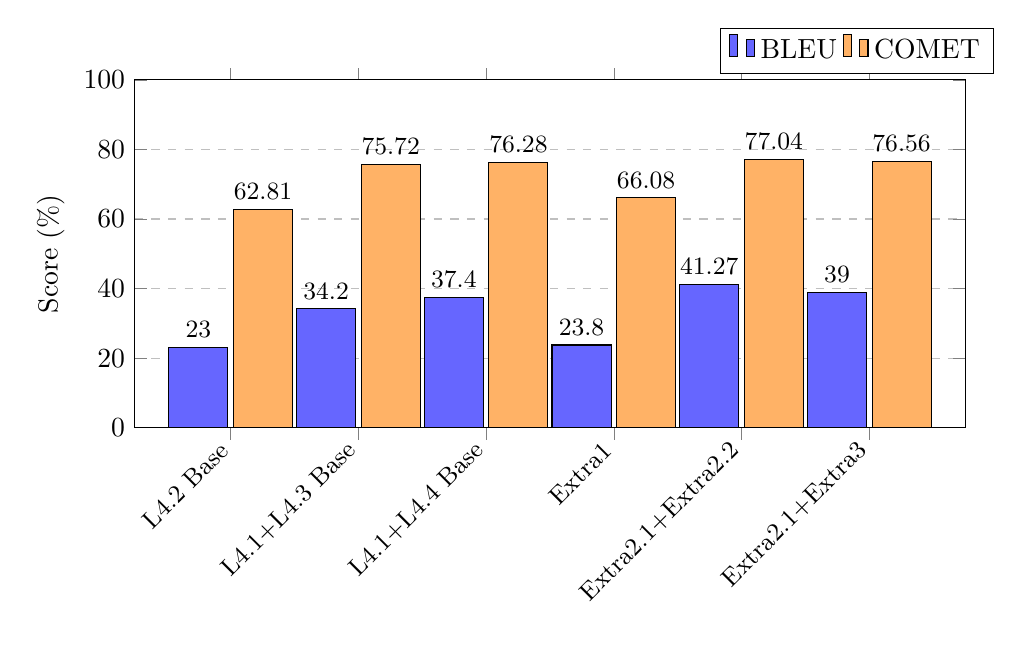
\begin{tikzpicture}
\begin{axis}[
    ybar,
    bar width=0.75cm,
    width=\textwidth,
    height=6cm,
    ylabel={Score (\%)},
    symbolic x coords={L4.2 Base, L4.1+L4.3 Base, L4.1+L4.4 Base, Extra1, Extra2.1+Extra2.2, Extra2.1+Extra3},
    xtick=data,
    x tick label style={font=\small, rotate=45, anchor=east},
    ymin=0,
    ymax=100,
    ymajorgrids=true,
    grid style=dashed,
    enlarge x limits=0.15,
    nodes near coords,
    nodes near coords align={vertical},
    every node near coord/.append style={font=\small},
    legend style={at={(0.87,1.15)}, anchor=north, legend columns=2},
]
% BLEU scores
\addplot[fill=blue!60] coordinates {
    (L4.2 Base, 23.0)
    (L4.1+L4.3 Base, 34.2)
    (L4.1+L4.4 Base, 37.4)
    (Extra1, 23.8)
    (Extra2.1+Extra2.2, 41.27)
    (Extra2.1+Extra3, 39.0)
};
\addlegendentry{BLEU}
% COMET scores
\addplot[fill=orange!60] coordinates {
    (L4.2 Base, 62.81)
    (L4.1+L4.3 Base, 75.72)
    (L4.1+L4.4 Base, 76.28)
    (Extra1, 66.08)
    (Extra2.1+Extra2.2, 77.04)
    (Extra2.1+Extra3, 76.56)
};
\addlegendentry{COMET}
\end{axis}
\end{tikzpicture}
\caption{Comparación de métricas BLEU y COMET obtenidas en las traducciones completas.}
\label{fig:resultados_finales}
\end{figure}

Se observa que las traducciones \textit{end-to-end} con Whisper (Ejercicio L4.2 Base y Extra 1) no han conseguido resultados competitivos en comparación con las traducciones en cascada. Lo más eficaz ha sido la traducción en cascada con MADLAD sin \textit{finetuning} (Ejercicio extra 2.1 + Extra 2.2), que ha conseguido los mejores resultados tanto en BLEU (41.27\%) como en COMET (77.04\%) usando el experimento 2 con normalización. Aunque el \textit{finetuning} (Extra 3) ha mejorado con respecto a los resultados base, no ha superado los resultados obtenidos con MADLAD sin ajuste fino, demostrando que el modelo base con una configuración adecuada de decodificación puede ser más efectivo que un modelo ajustado.

Viendo el BLEU y COMET obtenidos en las transcripciones automáticas en cascada, se concluye que el mejor método ha sido:
\begin{itemize}
  \item Transcribir el audio usando el método del experimento 3 con normalización del Extra2.1.
  \item Y traducir el texto aplicando el experimento 2 con normalización del Extra2.2.
\end{itemize}

%%%%%%%%%%%%%%%%%%%%%%%%%%%%%%%%%%%%%%%%%%%%%%%%%%%%%%%%%%%%%%%%%%%%%%%%%%%%%%%
%                                                                             %
%                                BIBLIOGRAFIA                                 %
%                                                                             %
%%%%%%%%%%%%%%%%%%%%%%%%%%%%%%%%%%%%%%%%%%%%%%%%%%%%%%%%%%%%%%%%%%%%%%%%%%%%%%%
\cleardoublepage
\printbibliography

%%%%%%%%%%%%%%%%%%%%%%%%%%%%%%%%%%%%%%%%%%%%%%%%%%%%%%%%%%%%%%%%%%%%%%%%%%%%%%%
%                                                                             %
%                                 APÉNDICES                                   %
%                                                                             %
%%%%%%%%%%%%%%%%%%%%%%%%%%%%%%%%%%%%%%%%%%%%%%%%%%%%%%%%%%%%%%%%%%%%%%%%%%%%%%%

\APPENDIX


%%%%%%%%%%%%%%%%%%%%%%%%%%%%%%%%%%%%%%%%%%%%%%%%%%%%%%%%%%%%%%%%%%%%%%%%%%%%%%
%                       APÉNDICES                                            %
%%%%%%%%%%%%%%%%%%%%%%%%%%%%%%%%%%%%%%%%%%%%%%%%%%%%%%%%%%%%%%%%%%%%%%%%%%%%%%

% \chapter{Apéndice correspondencia notebooks}
% \label{appendix:notebooks}
% ...

%%%%%%%%%%%%%%%%%%%%%%%%%%%%%%%%%%%%%%%%%%%%%%%%%%%%%%%%%%%%%%%%%%%%%%%%%%%%%%%
%                              FIN DEL DOCUMENTO                              %
%%%%%%%%%%%%%%%%%%%%%%%%%%%%%%%%%%%%%%%%%%%%%%%%%%%%%%%%%%%%%%%%%%%%%%%%%%%%%%%
\end{document}

